\chapter{线性系统}
\section{线性系统}
\subsection{线性系统的基本定义}
线性系统将输入与输出映射起来,输出满足叠加性原则。

It's a mapping from inputs to outputs satisfies the principle of superposition.
\begin{figure}[H]
	\centering
	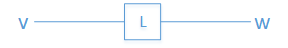
\includegraphics[width=0.4\textwidth]{assets/LinearSystem.png}
	\caption{线性系统}
\end{figure}

\begin{align*}
	L(v_1+V_2)  & =Lv_1+Lv_2   \\
	L(a\cdot v) & =a\cdot L(v)
\end{align*}

结合上面两个性质,有:
\begin{equation}
	L\ (\sum\limits_{i=1}^n\ a_i\cdot v_i)=\sum\limits_{i=1}^n\ a_i\cdot Lv_i
\end{equation}

你甚至可以将其延伸到无限领域:
\begin{equation}
	L\ (\sum\limits_{i=-\infty}^\infty\ a_i\cdot v_i)=\sum\limits_{i=1}^n\ a_i\cdot Lv_i
\end{equation}

虽然这样的话,我们需要对运算符$L$做一些额外的假设。

例如,抽样可以视作一个线性系统。

\subsection{离散有限维线性系统}
\subsubsection{矩阵的乘法}
矩阵与向量的乘法满足叠加性原则:
\begin{equation}
	(A\cdot \vec{v})_i=\sum\limits_{j=i}^m\ a_{ij}\cdot \vec{v}_j
\end{equation}

另外,毫无疑问,矩阵的乘法也符合叠加性原则,此处略去验证步骤。
\subsubsection{具有特征向量的线性系统矩阵}
如果对于某个线性系统矩阵$A$,有特征向量$v_1,v_2,\cdots,v_n$,他们相应的特征值为$\lambda_1,\lambda_2,\cdots,\lambda_n$,这些特征向量就形成了对于所有输入的一组基。这句话的意思是:对于任意的输入$v$都能用下式来表达:
\begin{equation}
	v = \sum_{i=1}^{n}\alpha_iv_i
\end{equation}

那么,线性系统矩阵$A$对任意输入$v$的作用就可以表达为:
\begin{equation}
	Av = \sum_{i=1}^{n}A(\alpha_iv_i) = \sum_{i=1}^n\alpha_i(Av_i) = \sum_{i=1}^n \alpha_i\lambda_iv_i
\end{equation}

矩阵乘法不仅仅是有限维线性系统的一个好例子,它还是唯一的例子,也就是说在一个有限维度空间内的任何线性算符都可以被理解为矩阵乘法。

\begin{quote}
	我们举一个求微分的例子:

	有输入为小于等于$n$阶的多项式:
	$$
		a_0+a_1x+a_2x^2+…+a_nx^n
	$$

	现在我们需要对该输入进行线性运算,线性算符为微分,即:
	$$
		L = \frac{d}{dx}
	$$

	由于输入共有$n+1$项,所以把$L$当作一个$(n+1)\times (n+1)$的矩阵,我们需要求出$L$的这个矩阵具体是什么。根据我们对微分的理解,可以写成如下等式:
	$$
		L\cdot \begin{bmatrix} a_0\\  a_1\\  a_2\\  \vdots\\  a_n \end{bmatrix} = \begin{bmatrix} a_1\\  2a_2\\  \vdots\\  na_n\\  0 \end{bmatrix}
	$$

	那么矩阵$L$为:
	$$
		L=\begin{bmatrix} 0 &1  &0  &  &  &\cdots   &0 \\  0 &0  &2  &0  &  &\cdots   &0 \\  0 &0  &0  &3  &0  &\cdots   &0 \\  0 &0  &0  &0  &4  &\cdots   &0 \\  \vdots &\vdots  &\vdots  &\vdots  &\vdots  &\cdots   &\vdots \\  0 &0  &0  &  &  &\cdots   &n \\  0 &0  &0  &0  &  &\cdots   &0  \end{bmatrix}
	$$
\end{quote}
\subsection{连续无限维线性系统}
\subsubsection{核函数的积分}
$$
	Lv(x) = \displaystyle{ \int_{-\infty}^{\infty}k(x,y)v(y)dy }
$$

其中积分为线性的,积分符合叠加性原则,即:
\begin{align*}
	  & L(a_1v_1(x)+a_2v_2(x))                                                             \\
	= & \int_{-\infty}^{\infty}k(x,y)\left(a_1v_1(y)+a_2v_2(y)\right)dy                    \\
	= & a_1 \int_{-\infty}^{\infty}k(x,y)v_1(y)dy+a_2\int_{-\infty}^{\infty}k(x,y)v_2(y)dy \\
	= & a_1Lv_1(x)+a_2Lv_2(x)
\end{align*}

因此对输入函数与核函数的积分必然也是一个线性系统。
\subsubsection{另外一种理解方式}
我们也可以用另外一种方式去理解上述的积分线性系统:
\begin{enumerate}
	\item 把输入函数$v(y)$当作无限维度的列矩阵,yy为下标;
	\item 把核函数$k(x,y)$当作无限维度的线性系统矩阵,$x,y$分别为行、列下标;
	\item $K(x,y)v(y)$代表了$k$的$k_{xy}$项与$v$的$v_y$项的乘积;
	\item $\int_{-\infty}^{\infty}k(x,y)v(y)dy$代表了$k$的第$x$行与整个$v$列矩阵的内积,最终会得到以$x$为下标的无限维度列矩阵$Lv(x)$。
\end{enumerate}
\subsubsection{一些特殊的核函数}
\begin{enumerate}
	\item 线性系统矩阵是对称的$A^T=A$
	      他们在核函数上的表现为:
	      \begin{align*}
		      k(x,y)=k(y,x) \\
		      k(x,y)=\overline{k(y,x)}
	      \end{align*}
	\item 傅立叶变换
	      $$
		      \mathcal{F}f(s)=\int_{-\infty}^\infty\ e^{-2\cdot\pi\cdot i\cdot s\cdot t}\cdot f(t)\ dt
	      $$
	      其中核函数为:$k(s,t)=e^{-2\cdot\pi\cdot i\cdot s\cdot t}$,它也满足对称性。
	\item 卷积
	      $$
		      h*v = \int_{-\infty}^{\infty}\ h(x-y)\cdot v(y)\ dy
	      $$

	      以线性系统的角度来分析,即:
	      $$
		      L\ v = \int_{-\infty}^{\infty}\ h(x-y)\cdot v(y)\ dy
	      $$

	      这里的核函数为$h(x−y)$,特殊的是该核函数并非基于单独的$x,y$,而是基于他们的差值$x−y$。这个特殊的性质导致了所谓的平移不变性或时间不变性。

	      当我们令$x,y$同时移动$a$,即:
	      \begin{align*} x\ &\rightarrow \ x-a \\ y\ &\rightarrow \ y-a \\ (x-y)\ &\rightarrow \ (x-a)-(y-a)=x-y \end{align*}

	      对核函数积分不仅仅是连续无限维度线性系统的一个好例子,他还是唯一的例子,也就是说,任意在练习无限维度空间内的线性系统都能通过对核函数的积分来表示
\end{enumerate}
\section{脉冲响应}
\subsection{级联线性系统(Cascading Linear System)}
\begin{figure}[H]
	\centering
	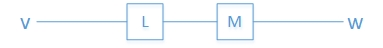
\includegraphics[width=0.4\textwidth]{assets/inpulse.jpg}
	\caption{描述}
\end{figure}
如果$L$与$M$都是线性的,有:
$$
	w=M\ L\ v
$$

下面讨论特殊的情况:
$$
	L\ v(x)=\int_{-\infty}^\infty\ k(x,y)\cdot v(y)\ dy
$$
在连续无限维空间中:
$$
	M\ L\ v(x)= \int_{-\infty}^\infty\ M_x\ k(x,y)\cdot v(y)\ dy
$$

我们做一个近似:
$$
	\int_{-\infty}^\infty\ k(x,y)\cdot v(y)\ dy\approx \sum\limits_i\ k(x,y_i)\cdot v(y_i)\ dy_i
$$

因此:
\begin{align*}
	        & M_x(\sum\limits_i\ k(x,y_i)\cdot v(y_i)\cdot \Delta y_i) \\
	=       & \sum\limits_i\ M_x(k(x,y_i)\cdot v(y_i)\cdot \Delta y_i) \\
	=       & \sum\limits_i\ M_x(k(x,y_i))\cdot v(y_i)                 \\
	\approx & \int_{-\infty}^\infty\ M_x(k(x,y))\cdot v(y)\ dy
\end{align*}

由于我们是对$x$做线性变换,因此$v(y_i)$和$\Delta y_i$都视作常量。
\subsection{脉冲相应的定义}
任何线性系统都由对核(函数)的积分得到,核(函数)就是该线性系统对脉冲函数的响应。

Any linear system is given by integration against a kernel (impulse response).

推导过程如下:

\begin{align*}
	  & v(x)                                     \\
	= & (\delta * v)(x)                          \\
	= & \int_{-\infty}^{\infty}\delta(x-y)v(y)dy \\
	  & (\delta\ shift\ property)
\end{align*}

那么线性系统有如下表示:

\begin{align*}
	  & L\ v(x)                                          \\
	= & L( \int_{-\infty}^{\infty}\ \delta(x-y)v(y)dy  ) \\
	= & \int_{-\infty}^{\infty}\ L_x\delta(x-y)v(y)dy
\end{align*}

令$k(x,y) = L_x\delta(x-y)$,则有:
$$
	Lv(x) = \int_{-\infty}^{\infty}\ k(x,y)\cdot v(y)\ dy
$$

其中$k(x,y)$是该线性系统的核函数,它由$L_x\ \delta(x−y)$得到,同时他也是该线性系统的脉冲响应。

脉冲响应的定义如下:

$\delta(x−y)$是位置在$y$上的脉冲,$L_x\ \delta(x−y)$表示了把脉冲输入到该线性系统,此时系统会做出响应,并输出脉冲响应$k(x,y)$。
\subsection{Schwartz核函数定理}
如果$L$是广义函数(分布)的一个线性算符,即$L$在符合叠加性原则的基础上将一个广义函数变换为另一个广义函数,那么就会存在唯一的核$k$,使得$L\ v=<k,v>$。
\subsection{傅立叶变换的脉冲响应}
当输入脉冲函数$\delta(x-y)$,傅立叶变换会输出:
$$
	h(x,y) = \mathcal{F}(\delta(x-y)) = e^{-2\pi ixy}
$$

另外,傅立叶变换的公式如下:
$$
	\mathcal{F}f(x) =  \int_{-\infty}^{\infty}e^{-2\cdot \pi\cdot  i\cdot x\cdot y}f(y)dy
$$

它的核函数为:
$$
	k(x,y) = e^{-2\cdot \pi\cdot  i\cdot x\cdot y}
$$

我们注意到,核函数与脉冲响应式一样的,其中有如下关系:

如果一个线性算符能表示成对于$k(x,y)$与输入函数乘积的积分形式,那么$k(x,y)$就是脉冲响应了。反过来说,如果我们能得到线性系统的脉冲响应,就能通过对脉冲响应和输入函数的乘积进行积分来表达该线性系统的线性算符。

\subsection{离散有限维线性系统的脉冲响应}
在连续无限维的线性系统中,脉冲响应是线性系统对输入脉冲$\delta(x-y)$的响应。在离散有限维线性系统也同样是对输入脉冲序列的响应,用矩阵乘法的表达如下:
\begin{align*}
	  & A\cdot \left[ \underline{\delta}_0,\underline{\delta}_1,\underline{\delta}_2,\cdots ,\underline{\delta}_{n-1} \right] \\
	= & A\cdot\begin{bmatrix} 1 &0  &0  &\cdots   &0 \\  0 &1  &0  &\cdots   &0 \\  0 &0  &1  &\cdots   &0 \\  \vdots &\vdots  &\vdots  &\cdots   &\vdots \\  0 &0  &0  &\cdots   &1  \end{bmatrix}=A
\end{align*}
\subsection{脉冲响应的例子——开关}
\begin{align*}
	L\ v = \Pi v
\end{align*}

它的脉冲响应为:
\begin{align*}
	  & h(x,y)                           \\
	= & L\delta(x-y) = \Pi(x)\delta(x-y) \\
	= & \Pi(y)\delta(x-y)                \\
	  & (\delta\ sampling\ property)
\end{align*}

对脉冲响应与输入函数乘积的积分会得到开关的线性算符:
\begin{align*}
	  & \int_{-\infty}^{\infty}h(x,y)v(y)dy                            \\
	= & \int_{-\infty}^{\infty}\Pi(y)\delta(x-y)v(y)dy                 \\
	= & \int_{-\infty}^{\infty}\delta(x-y)\left( \Pi(y)v(y) \right )dy \\
	= & \left(\delta * (\Pi v) \right )(x)                             \\
	  & (\delta\ shift\ property)                                      \\
	= & \Pi(x)v(x)
\end{align*}

这个结果证明了前面的结论是正确的。
\section{卷积、连续无限维线性时不变系统}
引入时移符号$\tau$:
$$
	\tau_a v(x) = v(x-a)
$$

假设有用卷积表达的线性系统如下:
$$
	L\ v = h*v
$$

如果我们对输入vv进行延时a:
\begin{align*}
	  & L\tau_a v(x)                                                   \\
	= & (h*\tau_av)(x)                                                 \\
	= & \int_{-\infty}^{\infty}h(x-y)v(y-a)dy                          \\
	= & \int_{-\infty}^{\infty}h(x-z-a)v(z)dz                          \\
	  & (letting\ z=y-a)                                               \\
	= & \int_{-\infty}^{\infty}\left(h(x-z)*\delta(x-a) \right )v(z)dz \\
	  & (\delta\ shift\ property)                                      \\
	= & \left(\int_{-\infty}^{\infty}h(x-z)v(z)dz \right )*\delta(x-a) \\
	= & (h*v)(x-a)                                                     \\
	= & \tau_a(h*v)(x)                                                 \\
	= & \tau_aLv(x)
\end{align*}

结果显示该线性系统输出的延时与输入的延时同为$a$,这被称为线性时不变系统(Linear Time Invariant System)。

结论是:

如果一个线性系统是由卷积给定的,那么他就是时不变的。


反过来也是成立的:

如果一个线性系统是时不变的,那么它一定是由卷积给定的。
证明过程如下:

任何连续无限维线性系统都有如下表示

$$
	Lv = \int_{-\infty}^{\infty}L_x\delta(x-y)v(y)dy
$$

我们令$h(x)=L_x\ \delta(x)$,就是线性系统对$\delta_0$进行脉冲响应。则有:
$$
	L_x\delta(x-y) = L_x(\tau_y\delta(x))
$$

如果$L$是时不变的,则输出与输入会有同一延时:
\begin{align*}
	  & L_x\delta(x-y)       \\
	= & L_x(\tau_y\delta(x)) \\
	= & \tau_y(L_x\delta(x)) \\
	= & \tau_yh(x) = h(x-y)
\end{align*}

即:
$$
	Lv = \int_{-\infty}^{\infty}h(x-y)v(y)dy
$$
\section{矩阵卷积、离散有限维线性时不变系统}
